\chapter{Распределение радиоресурсов: схема параллельного обучения для гетерогенных сетей малых станций стандарта LTE} \label{chapt2}

\section{Общее описание предметной области} \label{sect2_1}

Растущий спрос на поддержание высокого качества услуг беспроводных сотовых технологий создает реальную проблему для телекоммуникационных сетей новых поколений~\cite{TS36.300}. Одним из основных технических требований, предъявляемых к современным сотовым системам, является максимизация фактора повторного использования частот ~\cite{M.1645}. Дефицит лицензированного спектра безусловно приводит к перекрытию диапазонов частот и интерференции между сотами (Inter-Cell Interference, ICI). В сфере контроля и ликвидации интерференции осуществляется интенсивная научная деятельность. В промышленности эти усилия в основном отражаются в виде строгого статического разделения частот или реактивного (в отличие от активного) ручного управления доступным спектром.

Концепция малых сот считается одним из самых практичных способов увеличения общей пропускной способности системы. В этом подходе большое количество маломощных устройств (малые соты) используется для увеличения повторного пространственного использования частот и улучшения местного покрытия. Согласно определению консорциума Small Cell Forum, «малые соты — это управляемые оператором маломощные беспроводные точки доступа с интеллектуальным обслуживанием, работающие в лицензированном диапазоне радиочастотного спектра. К типам малых сот относятся фемтосоты, пикосоты, метросоты и микросоты. Размер сот увеличивается от фемтосот (наименьший) до микросот (наибольший)»~\cite{6171992}. Довольно часто малые соты развертываются без или с небольшим объемом радиопланирования от оператора сети. Для того, чтобы гарантировать в этом случае некоторый заданный уровень качества обслуживания, необходимо внедрять интеллектуальные механизмы управления радиоресурсами для малых сот. Эта концепция принципиально изменяет требования к работе системы сотовых сетей выбиваясь из традиционных представлений о структуре сетей сотовой связи ~\cite{6211486}. При использовании этого подхода большое количество маломощных устройств разворачивается с целью увеличения коэффициента повторного использования частот на выделенной области покрытия. В дополнение к обширному уплотнению, устройства теперь могут часто включаться и выключаться, что вызывает частые неконтролируемые изменения в структуре сети. Таким образом, применение традиционные подходов к контролю интерференции перестало быть возможным, поскольку они основаны на предположении о равномерном гексагональном построении сети и подходят только для централизованного управления базовыми станциями.

Вместе с ростом числа устройств увеличивается количество накладных расходов на передачу управляющей информации. В таких условиях использование централизованных решений становится гораздо менее эффективным, а распределенные алгоритмы для управления ресурсами являются более перспективными. Эффективное управление радиоресурсами и координация интерференции являются неотъемлимыми механизмами для успешного внедрения гетерогенных сетей с малыми сотами.   

В этой главе мы предлагаем подход к управлению передачами на базовых станциях, динамическую схему распределения ресурсов с распределенной двухуровневой процедурой обучения. Мы предполагаем использование только локальной информации с ограничением обмена информацией между соседними сотами. По замыслу, на каждой соте должен быть выработан уникальный набор правил распределения ресурсов, позволяюший всей системе оперативно прийти к оптимальной конфигурации. Мы иллюстрируем применение этой стратегии обучения для задачи выделения частотных поддиапазонов. Каждый обучаемый агент исследует окружающую среду, изучая реакции от конкурирующих агентов и невзаимодействующих базовых макро станций. Полученная информация затем используются, чтобы выбрать наиболее подходящее расписание передач. 

Предлагается рассмотреть распределенную мультиагентную стратегию, где малые соты локально контролируют использование ресурсов для максимизации общей пропускной способности системы. Основная идея заключается в том, чтобы возложить на каждую базовую станцию принятие решение об использовании радиоресурсов. При принятии решения должна учитываться занятость ресурсов окружающих сот. Основной вклад данной работы заключается в следующем. Предложен новый метод для координации интерференции в плотных гетерогенных сетях. Рассмотрены две типичные проблемы часто возникающие в параллельных схемах обучения - разрастание обучаемой модели и блокирование возможности обследования. Предложенный алгоритм осуществляет мониторинг местного уровня интерференции, использование ресурсов и выделяет блоки физических ресурсов оптимальным образом. Алгоритм является полностью распределенным, предполагается отсутствие связи между сотами. Алгоритм быстро адаптируется к изменению интерференции и внешних условий сети, что делает его очень практичным. Дополнительно изучается вопрос о скорости сходимости распределенного механизма и предлагается ряд промежуточных процедур для повышения эффективности обучения. Сходимость и быстродействие алгоритма исследуется путем имитационного моделирования. Результаты предложенного метода оцениваются при помощи моделирования для сети базовых станций LTE и сравниваются с рядом традиционных схем распределения ресурсов. Результаты моделирования на системном уровне показывают, что она обеспечивает значительное улучшение производительности системы для разнородного внедрения с невзаимодействующими агентами без ущерба для эффективности системы в целом.

\section{Описание технологии радиодоступа} \label{section2_2}


\subsection{Архитектура базовой станции} 
Ключевым элементом сети LTE, отвечающим за эффективное использование частотного спектра, является базовая станция. В данном разделе представлена архитектура базовой станции и рассмотрены компоненты, участвующие в процессе управления ресурсами.

\begin{figure}
  \center
  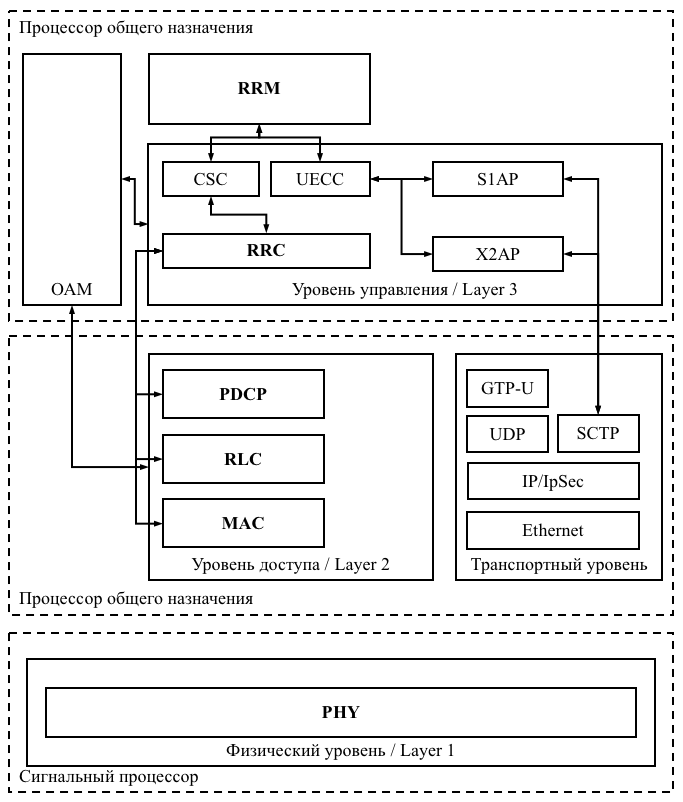
\includegraphics {image7}
  \caption{Архитектура базовой станции LTE. Источник \cite{Aricent}} 
  \label{img:image7}  
\end{figure}


Протокол PDCP (Packet Data Convergence Protocol) обеспечивает компрессию заголовков (ROHC), шифрование, сохранение порядка следования пакетов.

Протокол RLC (Radio Link Control) выполняет функции сегментирования, отброса дубликатов и сохранение порядка следования пакетов \cite{access2008and}. RLC функционирует в одном из трех режимов передачи: прозрачный (transparent mode, TM), передача без подтверждения (unacknowledged mode, UM) и передача с подтверждением (acknoledged mode, AM). В режиме AM поддерживаются специальные функции для повторной передачи данных.

Протокол RRC покрывает следующие функциональные области: передача системной информации, управление RRC соединением (RRC connection control). Сюда относятся процедуры создания, изменения и удаления RRC соединения, пейджинг, активацию защиты соединения, контроль ресурсов для передачи пользовательских данных. Также к этой области относится процедура хэндовера (handover) и конфигурация более низких уровней (PDCP, RLC, MAC).

Протокол RRC также осуществляет настройку измерений качества канала и отчетность на стороне пользовательского устройства, включая настройку и активацию периодов измерений (см. раздел \ref{ch_estimation}). Актуальность информации о состоянии канала напрямую влияет на эффективность передачи пользовательских данных.

Задача управления радиоресурсами решается протоколом RRM (Radio Resource Management). Сюда входит динамическое распределение ресурсов в восходящих и нисходящих направлениях, принятие решений о необходимости хэндовера и допуска пользователей к обслуживанию. Блок RRM также отвечает за ограничение использования спектра с целью контроля интерференции между базовыми станциями.

Задача протокола MAC (Media Access Control) заключается в выделении пользователям частотно временных ресурсов и поддержании гарантий качества обслуживания. Блок MAC также осуществляет выбор сигнально-кодовой конструкции, используемой для обслуживания пользователей.

\subsection{Физический уровень LTE} %\label{section5_2}

Обмен между базовой станцией и абонентским устройством осуществляется кадрами (в терминологии LTE – радиокадр) длительностью 10 мс (см. рис. \ref{img:image8}). Стандарт предусматривает две структуры кадров. Одна для случая частотного разделения каналов (Frequency Division Duplex — FDD), другая - для временного (Time Division Duplex — TDD).

В LTE используется OFDM модуляция, хорошо исследованная при разработке систем DVB, Wi-Fi и WiMAX. В стандарте LTE установлен стандартный шаг между поднесущими ∆f = 15 кГц, что соответствует длительности OFDM-символа 66,7 мкс.

Все временные параметры в спецификации LTE привязаны к минимальному временному кванту !!   =  1/(2048 ∙ ∆!), где ∆! – шаг между поднесущими, стандартно – 15 кГц. Таким образом, длительность радиокадра – 307200 ∙ !!. Отметим, что квант времени соответствует тактовой частоте 30,72 МГц, что кратно стандартной в 3G-системах частоте обработки 3,84 МГц (8×3,84 = 30,72) \cite{access2010lte}.

\begin{figure}
  \center
  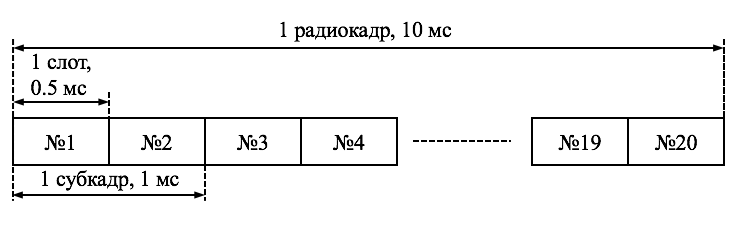
\includegraphics [width=\textwidth]{image8}
  \caption{Структура кадра LTE. Источник \cite{вишневский2009технология}} 
  \label{img:image8}  
\end{figure}


В каждом слоте абонентскому устройству назначается определенный диапазон канальных ресурсов в частотно-временной области – ресурсная сетка (см. рис. \ref{img:image9}). Ячейка ресурсной сетки (ресурсный элемент) соответствует одной поднесущей в частотной области и одному OFDM-символу – во временной. Группа ресурсных элементов образует ресурсный блок. Ресурсный блок – это минимальный квант радиоресурса, выделяемый абонентскому устройству планировщиком базовой станции. Ресурсный блок занимает 12 поднесущих (т.е. 180 кГц) и 7 или 6 OFDM-символов, в зависимости от типа циклического префикса – так, чтобы общая длительность слота составляла 0,5 мс. Число ресурсных блоков в ресурсной сетке зависит от ширины полосы канала и составляет от 6 до 100 (ширина частотных полос восходящего/нисходящего каналов в LTE – от 1,4 до 20 МГц). В новой версии стандарта LTE-A добавлена возможность агрегации до 5 полос шириной 20 МГц \cite{access2013lte}. О распределении ресурсов в каждом слоте базовая станция сообщает в управляющем канале, располагающемся в начале каждого субкадра.

\begin{figure}
  \center
  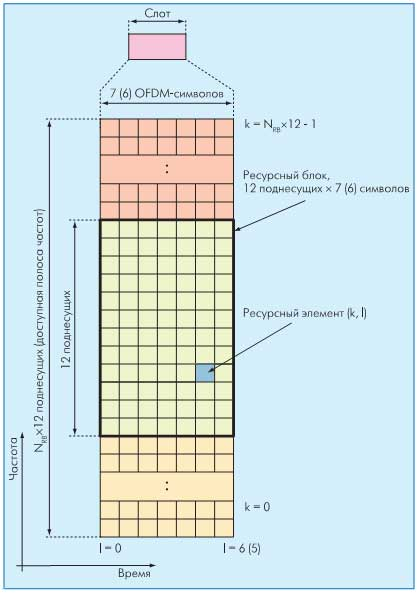
\includegraphics [width=\textwidth]{image9}
  \caption{Ресурсная сетка LTE при стандартном шаге поднесущих ∆f = 15 кГц. Источник \cite{вишневский2009технология}} 
  \label{img:image9}  
\end{figure}

Поднесущие модулируются посредством 4-, 16- и 64-позиционной квадратурной фазово-амплитудной модуляции (QPSK, 16-QAM или 64-QAM). Соответственно, один символ на одной поднесущей содержит 2, 4 или 6 бит информации. При стандартном префиксе символьная скорость составит 14000 символов/с. Сигнал с полосой 20 МГц содержит 100 ресурсных блоков или 1200 поднесущих, что дает общую скорость в канале от 33,6 до 100,8 Мбит/с.

Для повышения надежности передачи на физическом уровне стандарт LTE использует механизм HARQ (Hybrid Automatic Repeat Request). HARQ представляет собой комбинацию высокоскоростного помехоустойчивого кода и стандартного механизма ARQ \cite{access2008and}. Эта технология позволяет пользовательскому устройству запросить дополнительные проверочные биты при обнаружении ошибки декодирования.

\subsection{Оценка канала} \label{ch_estimation}

Для эффективного осуществления передачи данных базовая станция должна иметь оценку качества канала до обслуживаемого пользователя. Эта оценка используется для планирования расписания передач. Стандарт LTE предусматривает возможность запросить у пользователя отчет с оценкой качества канала. Для того чтобы задать формат отчетов о качестве канала, базовая станция посылает пользователю служебное сообщение RRC ConnectionReconfiguration \cite{access2012lte} с указанием следующих параметров:

При получении сообщения RRC ConnectionReconfiguration \cite{access2012lte} пользовательское устройство проводит измерения мощности пилотных сигналов соседних станций и через время равное reportInterval посылает их в отчете Measurement report. Эти величины называются RSRP (Reference Signal Received Power) \cite{access2010lte} и квантуется в соответствии с рисунком 10.

\section{Обзор методов координации интерференции в сотовых сетях}
%\blindtext


В данном разделе представлен обзор смежных работ в области управления радиоресурсами и координации интерференции в сотовых сетях. Существует множество исследований по данной теме, в особенности, на тему интерференции между макростанциями. На данный момент этот эффект является одним из основных сдерживающих факторов в сценариях с плотным развертыванием малых сот. В связи с этим в мире ведутся многочисленные исследовательские работы, посвященные различным вариантом управления ресурсами в разнородных сетях. Подробный обзор основных методов управления интерференцией, совместимых с LTE представлен в ~\cite{cite_overview}.

Для плотных неконтролируемых внедрений базовых станций задача управления интерференцией между сотами является более сложной, чем в традиционных операторских сотовых сетях. Один из перспективных методов управления радиоресурсами основывается на проведении предварительного исследовании радиоокружения, с целью выявления статистических данных об использовании ресурсов. Затем извлеченные данные могут быть использованы для непосредственного принятия решений (как в \cite{mab}) или (как, например, в \cite{q-learning}) для построения оптимальной схемы распределения ресурсов. В частности, в работе~\cite{q-learning} исследуется вопрос о самоорганизации и децентрализованном управлении интерференцией в сети фемтосот с целью разделения радиоресурсов между фемтосотами и макроокружением (сетью макро базовых станций и другими источниками интерференции). В этой работе рассмотрен многоагентный подход к обучению на основе распределенного Q-обучения (Q-learning). Малые соты меняют свою мощность передачи, чтобы максимизировать суммарную выходную мощность, в то время как суммарная интереференция макро пользователей в нисходящей линии связи поддерживается в заданных пределах.

В \cite{mp-qlearning} и \cite{fzq-learning} авторы предлагают другие схемы на основе Q-обучения и демонстрируют значительный выигрыш по сравнению с обычными методами повторного использования частот с точки зрения пропускной способности пользователей сотовой сети. Однако, эти методы устанавливают жесткие требования к качеству канала обратной связи и менее эффективны с точки зрения времени сходимости в динамичных случаях с гибким трафиком. 

В \cite{mab} предложен подход с использованием машинного обучения с подкреплением, где базовые станции автономно выбирают наиболее эффективную схему использования спектральных ресурсов из заранее заданного набора. Это позволяет гибко управлять компромиссом между фазой изучения окружающей среды и фазой использования накопленной информации. Похожие схемы с возможностью автоконфигурации и самооптимизации также были представлены в \cite{local-area}, где алгоритм позволяет сотам динамически выбирать начальные участки спектра и опирается на механизмы контроля мощности. Управление интерференцией между сотами было также изучено в \cite{on-uplink}, где авторы предложили схему планирования с фиксированными вероятностями выбора ресурсных блоков. В данном случае, сложность предлагаемых стохастически схем управления радио ресурсами является относительно низкой, поскольку они предполагают децентрализованный подход и требуют только ограниченный объем передачи управляющей информации. Однако, эти схемы могут быть неэффективными при рассмотрении сетей малых сот большого размера.
Еще один интересный децентрализованный подход был предложен в ~\cite{1666484}, где проблема распределения каналов сводится к задаче раскраски графа. Единственная информация, необходимая алгоритму, - обратная связь по уровню интерференции на выбранном канале. В~\cite{Duffy:2008:CAD:1377038.1377164} и ~\cite{4177619}сложность и скорость сходимости изучены для класса децентрализованных алгоритмов раскраски. Отметим, что проблема, рассматриваемая в данной главе, не может быть сведена к раскраске графа, так как соты могут находиться на одном и том же поддиапазоне, а границы частот поддиапазонов не фиксируются.
В то время как описанные решения обеспечивают подходы к управлению распределением ресурсов, они не учитывают ряд важных моментов, рассматриваемых далее в работе. Предлагается рассмотреть метод управления интерференцией, сделав упор на исследование нескольких ощутимых недостатков мультиагентного обучения. Основной проблемой является рассогласование между состоянием всей системы и поведением каждого агента в отдельности. В перспективе исследования скорости сходимости система имеет два состояния - состояние ''разведки'', где изучение окружающей среды движет систему к стабильному состоянию, и состояние ''эксплуатации'' - стабильное состояние, где эффективность обучения низка в связи с необходимостью сохранить стабильность системы. Недостатком такого подхода является то, что система интенсивно изучает среду в одном состоянии (где поведение агентов определяется, главным образом, исследованием поведения окружения), а затем работает в другом состоянии (определяемым эксплуатационным поведением агентов). В этой главе мы предлагаем первоначально заставить группу агентов вести себя уникальным образом, чтобы добавить больше смысла в процесс обучения. Мы также изучаем еще одну проблему схемы обучения, которая заключается в разрастании пространства состояний обучаемой модели с увеличением количества поддиапазонов.
Цель этого исследования заключается в получении схемы управления интерференцией посредством распределения частотных ресурсов с применением нескольких новых усовершенствований поведения обучаемых агентов с акцентом на их сосуществовании в плотной сотовой сети.

\section{Постановка задачи распределения ресурсов}
\subsection{Архитектура системы}
В этой главе мы рассматриваем сотовые сети технологии LTE/LTE-А с разнородным внедрением базовых станций, таких как макросоты и малые соты, как показано на Рис.~\ref{fig:architecture}. Малые соты обычно используются для улучшения покрытия в помещениях и для повышения общей пропускной способности в густонаселенных районах. Основной упор в данном разделе сделан на сосуществование малых сот с макросредой и некооперативными группами малых сот.

\begin{figure}
    \centering
    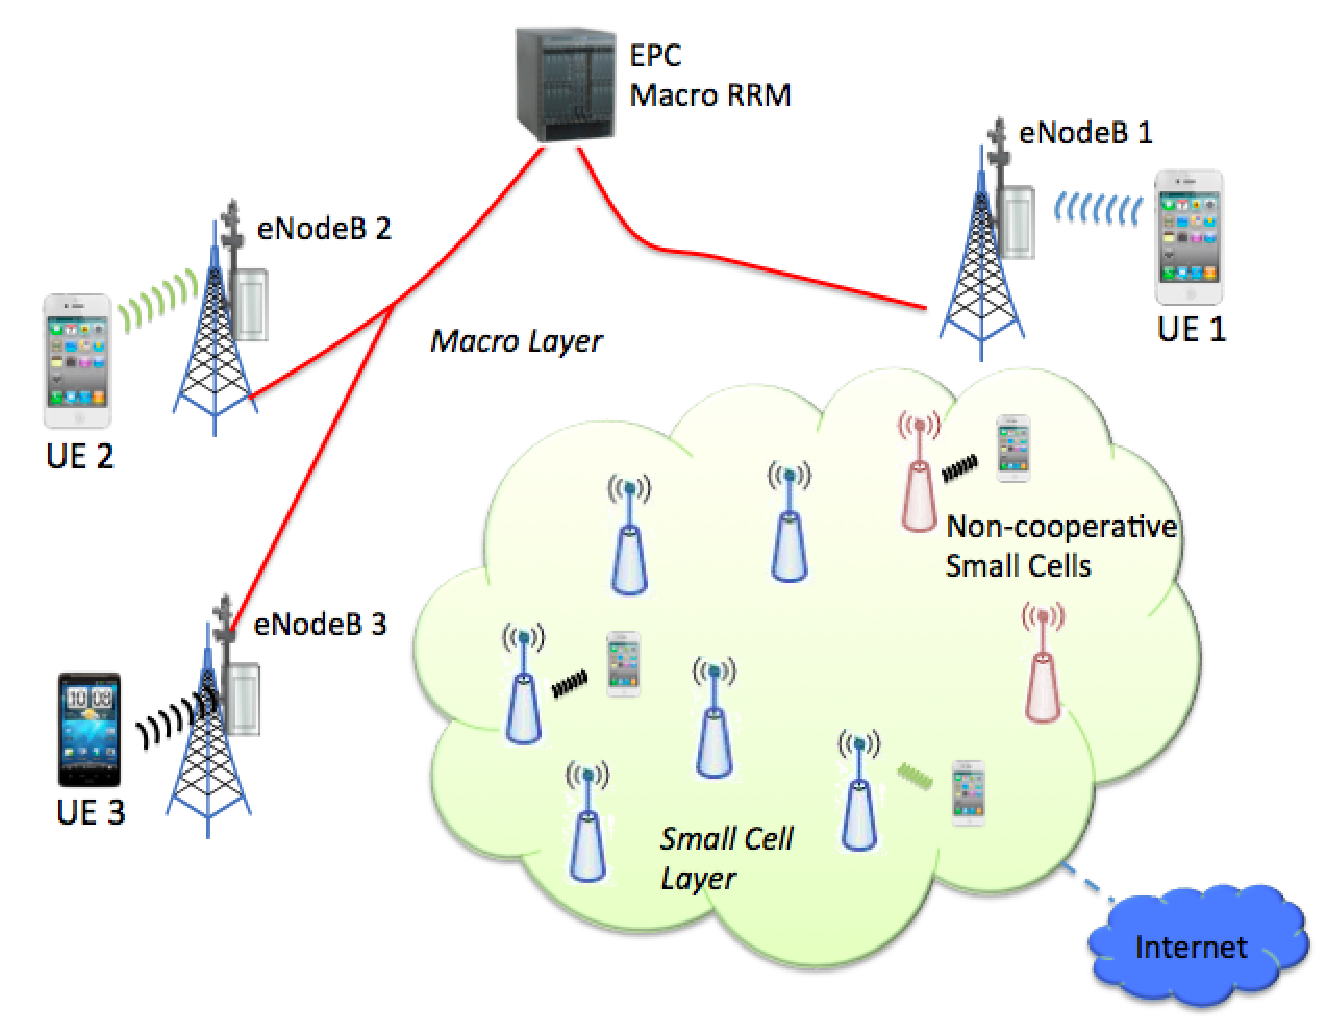
\includegraphics[width=8cm]{gcimages/architecture}
    \caption{Архитектура сети: макро уровень и уровень малых сот (кооперативные и некооперативные)}
    \label{fig:architecture}
\end{figure}

Рис.~\ref{fig:architecture} иллюстрирует типичный сценарий развертывания гетерогенных сетей~\cite{6824744}, которые обычно встречаются на практике. Они состоят из следующих элементов:

\begin{itemize}
\item[$\cdot$] Базовые макро станции (или eNodeB), которые используются для обеспечения основного покрытия сотовой сети. Базовые станции обычно конфигурируются по заранее подготовленным схемам, полученной на предварительном этапе радио-планирования. Качество покрытия базовых макро станций обычно ухудшается на границах соты и в помещениях из-за потерь сигнала и многолучевого замирания. 
\item[$\cdot$] Малые соты (HeNBs) - базовые станции малой дальности, которые в основном развернуты внутри помещений. Малые соты преимущественно развертываются без предварительного согласования и эксплуатируются без контроля со стороны оператора.
\item[$\cdot$] Некооперирующие соты - отдельный класс сетевых элементов, статически настроенные сотовым оператором или по какой-то причине действующие в рамках иных наборов правил, нежели рассматриваемые малые соты. В данной работе эти агенты (наряду с другими источниками помех) образуют ''поведение макросреды''.
\item[$\cdot$] Абонентское оборудование (UEs) - здесь мы не делаем различий между пользователями макросот и малых сот. Мы предполагаем, что пользователя всегда обслуживают базовая станция с самым сильным сигналом (что в большинстве случаев является верным предположением на практике)
\item[$\cdot$] Транспортная инфраструктура: базовые макро станции подключаются к пакетному ядру оператора (ЕРС) через выделенную линию, тогда как малые соты соединены через интернет. Отстутсвие прямой связи между ними делает распределенное алгоритмы управления более практичным для таких систем.
\end{itemize}

\subsection{Системные требования}
В этой главе мы предъявляем следующие требования:
\begin{enumerate}
\item алгоритм должен адаптироваться к различным схемам развертывания, условиям макросреды и типам трафика~\cite{TS36.300}.
\item управление системой должно происходить без вмешательства или предварительной конфигурации (требование самоорганизации)~\cite{TS36.902}.
\item отсутствие связи с посторонними агентами, чтобы избежать проблем с качеством транспортной сети и несовместимостью с проприетарными интерфейсами.
\item скорость сходимости алгоритма должна быть сопоставима с типичной скоростью изменений в системе.
\end{enumerate}

\subsection{Схема управления}
\begin{figure}
    \centering
    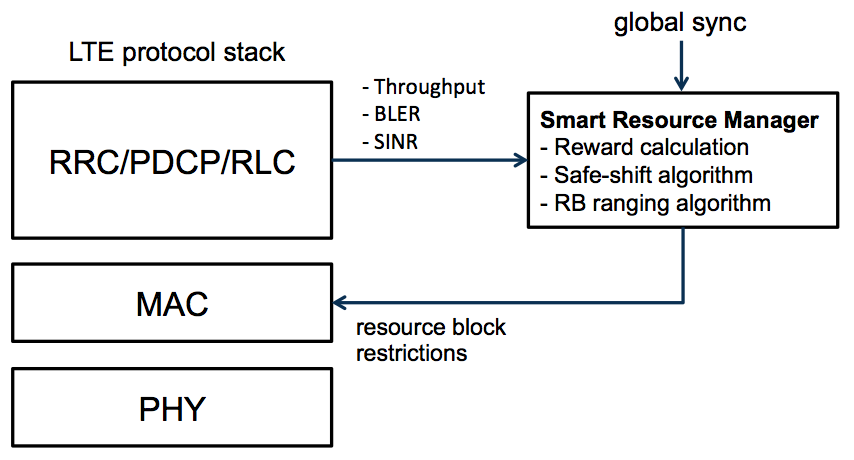
\includegraphics[width=8cm]{gcimages/algo_arch}
    \caption{Структура алгоритма и место в стеке протоколов LTE: PHY - физический уровень, MAC - уровень управления доступом к среде, RRC/PDCP/RLC - верхние уровни стека LTE}
    \label{fig:algo_arch}
\end{figure}

На Рис.~\ref{fig:algo_arch} представлена упрощенная структура алгоритма в стеке протоколов сети LTE. Можно заметить, что входящие или исходящие каналы управления не используются. Таким образом предлагаемое решение не налагает каких-либо требований на качество канала между базовыми станциями и выполняется локально на каждой малой соте.
Общий принцип алгоритма заключается в следующем. Основываясь на статистике производительности слоя L2~\cite{TS36.300} (например, BLER, спектральная эффективность) каждая малая сота локально принимает решение об использовании ресурсных блоков на последующем периоде времени. Единственный внешний входящий канал управления - глобальный источник точного времени. Он используется для выполнения синхронных операций (безопасный сдвиг) в пределах группы малых сот. После принятия решения о распределении ресурсов в каждой соте, выбранные ресурсные блоки  распределяются между пользователями базовой станции на уровне доступа к среде.

\subsection{Схема распределения радиоресурсов}
В этой части мы рассмотриваем разнородные сети LTE состоящие из множества малых сот, сосуществующих с окружающими базовыми макро станциями. Базовые макро станции и малые соты работают в одном частотном диапазоне, чтобы увеличить повторное использование пространственной частоты.

Для координации интерференции между соседними сотами каждая малая сота автономно принимает решения о распределении частот. Весь доступный частотный диапазон разбивается на ряд поддиапазонов $b_{j}$, где $j=1, .., N$ и $N$ - общее количество поддиапазонов. Распределение ресурсов внутри каждой базовой станции осуществляется планировщиком с алгоритмом пропорционального справедливого разделения (Proportional fair).

В момент времени $t$ автономный агент должен решить, какой поддиапазон $b(t+1)$ из имеющегося спектра доступен для использования на следующем временном промежутке $t+1$. Мы предлагаем схему обучения, состоящую из двух уровней (см. Рис.~\ref{fig:algo_arch}):

\begin{itemize}
\item[$\cdot$] параллельное обучение с подкреплением~\cite{4445757}, с $N\times N$ матрицей перехода $T(t)$. Она определяет вероятность перехода агента из поддиапазона $i$ в поддиапазон $j$ в момент времени $t$. Элементы матрицы периодически обновляются полученными наградами $RW_{ij}(t) = e^{(C_i(t-1) - C_j(t))}$, где $C_j(t)$ - достигаемая пропускная способность или количество пользователей с удовлетворенными требованиями к качеству обслуживания в момент времени $t$ при использовании поддиапазона $j$.
\item[$\cdot$] исследование макросреды (см. разд.~\ref{sec:safe_shift}), верхний уровень алгоритма с исследованием макросреды без вмешательства, где обучаемые агенты синхронно выполняют согласованную смену схемы использования ресурсов (безопасный сдвиг). $RW_{ij}(t_{sh})$ рассчитывается точно так же, как $RW_{ij}(t)$, но во время этапа безопасного сдвига. Этот шаг отвечает за обеспечение сосуществования с невзаимодействующими агентами и исследования макросреды.
\end{itemize}

Матрица перехода $T$ определяет вероятность перехода из поддиапазона $i$ к поддиапазону $j$. Значения $T_{ij}(t)$ и $T_{ij}(t_{sh})$ обновляются на каждой итерации (каждую 1 мс) на основе функции вознаграждения как описано в~(\ref{eq:tm_update}).
\begin{equation}
    \label{eq:tm_update}
    T_{ij}(t) = (1-\alpha-\beta)T_{ij}(t-1) + \alpha RW_{ij}(t) + \beta RW_{ij}(t_{sh})
\end{equation}
\begin{equation}
    \label{eq:tm_update_c}
    RW_{ij}(t) = e^{(C_i(t-1) - C_j(t))}
\end{equation}
где:

\begin{itemize}
\item[$\cdot$]$ \alpha$ - коэффициент обучения, определяющий скорость сходимости алгоритма и соотношение этапов исследования и эксплуатации. Оптимальное значение для этого параметра подбирается экспериментально в ходе симуляций.
\item[$\cdot$] $\beta$ - коэффициент обучения ($\beta < \alpha$) для макросреды, определяющий скорость сходимости алгоритма верхнего уровня.
\end{itemize} 

В то время как соты не имеют одинаковых знаний об уровне занятости/интерференции каждого поддиапазона, матрица перехода $T$ обновляется независимо для каждой соты. В определенной степени, это может привести к уменьшению скорости сходимости алгоритма. Моделирование показывает, что этим поведением можно эффективно управлять с помощью тонкой настройки коэффициентов обучения. В следующем разделе предложен дополнительный метод для повышения скорости сходимости алгоритма.

\subsection{Исследование макросреды: алгоритм безопасного сдвига}
\label{sec:safe_shift}
Любой агент в каждый момент времени наблюдает ответ окружающей среды $\gamma = \gamma^{CL} + \gamma^{ML}$, который состоит из двух частей: $\gamma^{CL}$ - компонент, определяемый поведением соседних агентов, а $\gamma^{ML}$ - независимый компонент, определяемый слоем макросреды.
Рисунок~\ref{fig:channel_exploration_blocked} иллюстрирует простой случай так называемой блокировки канала, где этап исследования окружающей среды $\gamma^{ML}$ агентом №2 заблокирован компонентой $\gamma^{CL}$, обусловленной выбором диапазона агента №1. Аналогичным образом на практике подавляющее большинство попыток разведки будут заблокированы ответом канала $\gamma_b^{CL}$ соседей. 

\begin{figure}
    \centering
    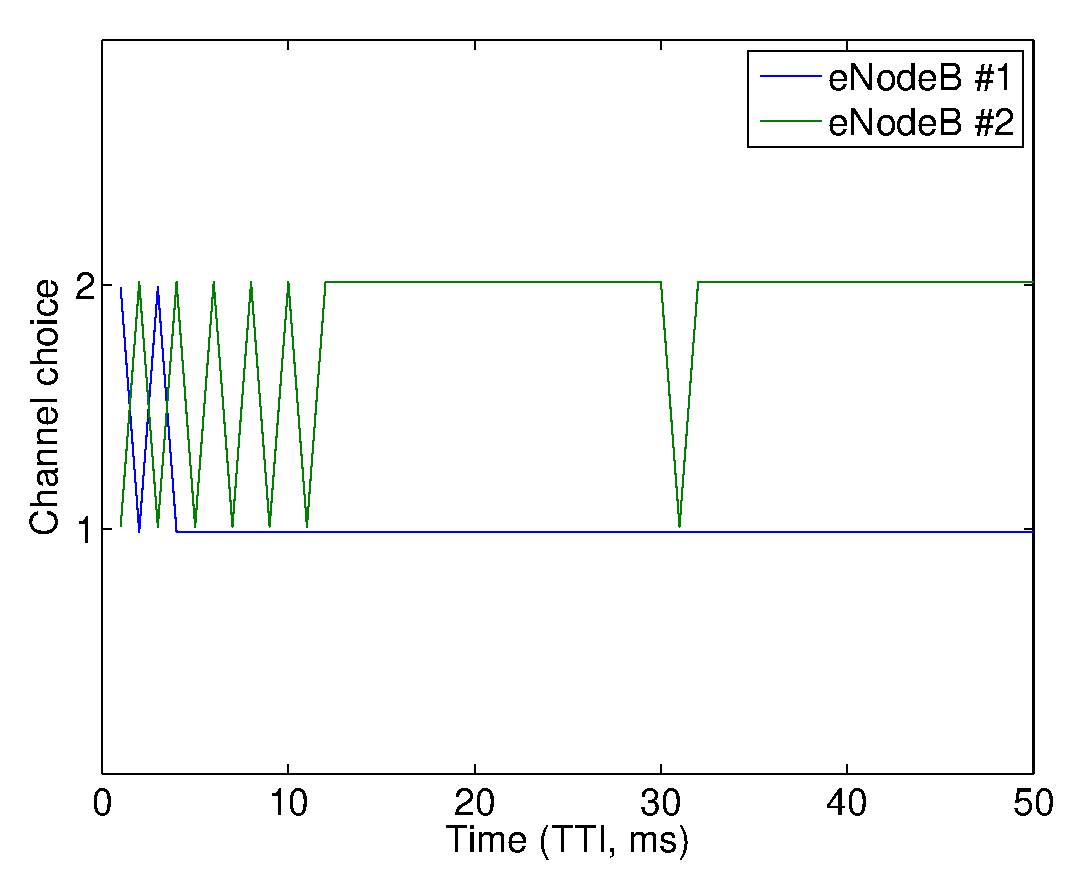
\includegraphics[width=8cm]{gcimages/channel_exploration_blocked}
    \caption{Пример эффекта блокировки канала. Оба частотных диапазона заблокированы.}
    \label{fig:channel_exploration_blocked}
\end{figure}

Чтобы побороть описанный эффект мы заставляем каждого агента изучать ответ макросреды $\gamma_b^{ML}$ в пределах каждого параллельного этапа обучения $t$ - процедуры безопасного сдвига. В рамках этой процедуры каждый агент последовательно изучает поддиапазоны в следующем порядке: ${(b_{t+1}+i)~mod~N}, i=1..N$. Очевидно, что это изменение не повлияет на компонент ответа $\gamma^{CL}$, так как агенты на пересекающихся поддиапазонах в момент времени $t$ по-прежнему используют те же поддиапазоны в момент времени ${t+1}$. В то же время компонент $\gamma^{ML}$ базового ответа окружающей среды изменяется.

Изучая отличия ответов окружающей среды $\gamma_b$, мы можем скорректировать оценки величин $\gamma_b^{ML}$ и $\gamma_b^{CL}$ для каждого агента в отдельности. Чтобы сохранить свойство локальности алгоритма, мы предлагаем управлять моментом запуска процедуры безопасного сдвига для каждого агента при помощи источника глобального времени. Значения функции вознаграждения при процедуре безопасного сдвига учитываются в соответствующей статистике для поддиапазонов в качестве отдельного компонента (см. формулу~\ref{eq:tm_update}). В результате обновления условия $\beta RW_{ij}(t_{sh})$, обучаемые агенты должны выбрать поддиапазоны с лучшим ответом макросреды.

Следующий эксперимент иллюстрирует простой пример процедуры безопасного сдвига. Рассмотрим случай двух малых сот разделяющих два частотных поддиапазона, где один из поддиапазонов занят невзаимодействующим агентом (например, базовая макро станция). После схождения процесса обучения малые соты 1 и 2 используют подздиапазоны 2 и 1 соответственно, каналы блокируются для исследования. Пусть поддиапазон 1 также занимает базовая макро станция или невзаимодействующий агент. Результат влияния процедуры безопасного сдвига на общую пропускную способность сети представлен на рис.~\ref{fig:safe_shift_overal_throughput}, где сдвиги производятся в моменты времени $t_1=200$ мс и $t_2=400$ мс. Этот шаг не влияет на взаимную интерференцию между агентами, но измененяет уровень помех от макросреды. Прирост около $10\%$ достигается без необходимости возобновления параллельного обучения для обоих агентов.

\begin{figure}
    \centering
    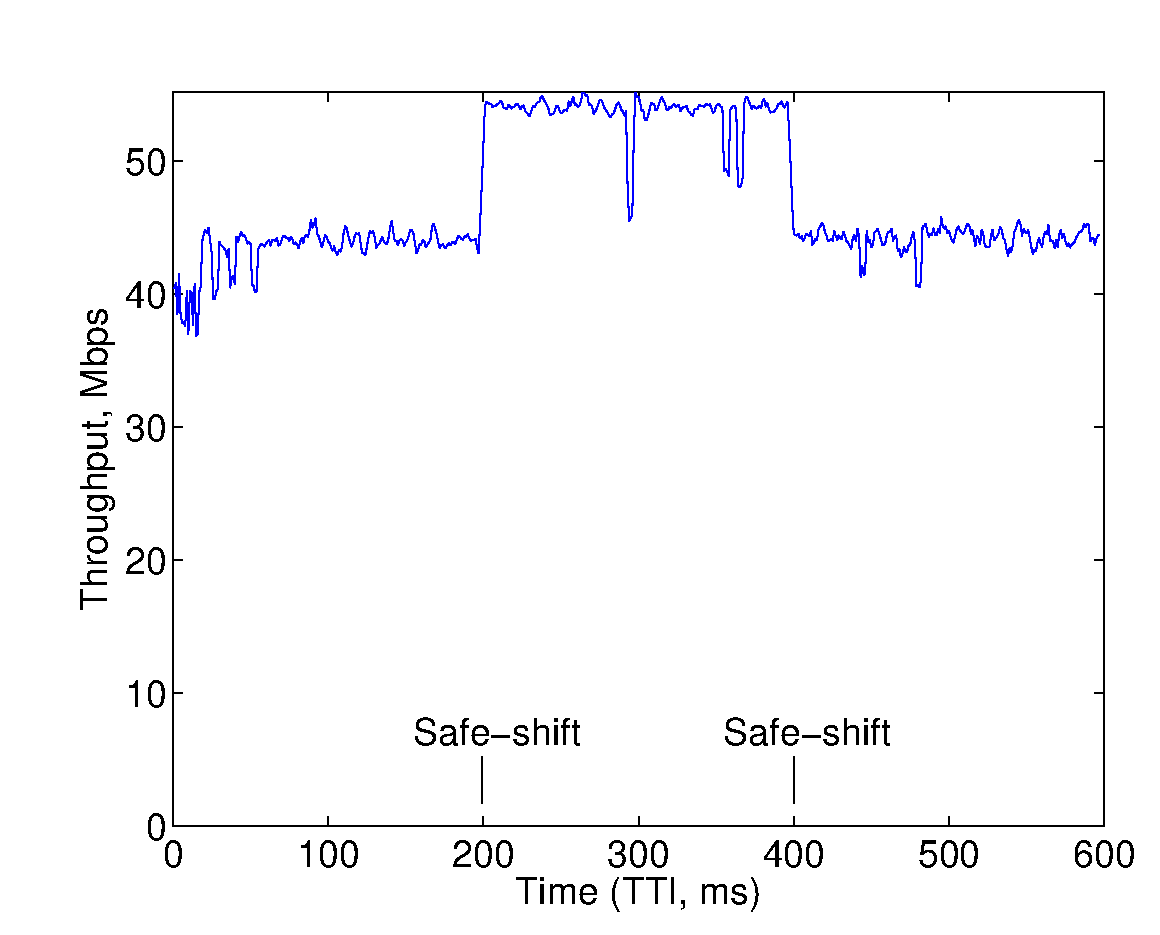
\includegraphics[width=8cm]{gcimages/overal_throughput}
    \caption{Прирост пропускной способности. Процедура безопасного сдвига инициирована в моменты времени $t_1=200$ мс и $t_2=400$ мс }
    \label{fig:safe_shift_overal_throughput}
\end{figure}

\subsection{Исследование скорости сходимости, выкалывание множества состояний}
В процессе обучения агенты постоянно изменяют свое состояние. Это в свою очередь инвалидирует стратегии других агентов, делая исходные условия, на которых они построены, устаревшими. Общий подход к этой проблеме заключается в том, чтобы считать этот эффект частью динамично изменяющейся среды. Однако, это предположение ослабляется в случае параллельного обучения множества агентов, где поведение динамической среды в большей степени определяется самими агентами.
Для того, чтобы преодолеть определяющую роль случайного исследования в структуре окружающей среды, мы предлагаем следующий способ. Идея в том, чтобы предварительно заставить агентов вести себя уникальным образом. В этом случае даже в процессе обучения посредством случайного исследования агенты могли бы получать статистически значимые наблюдения о поведении соседних агентов. Для этого мы предлагаем случайно выколоть часть $p$ $(p< 1)$ элементов матрицы перехода $TM_{ij}$ для каждого агента. Ожидается, что этот метод значительно уменьшит время сходимости процесса обучения.


\begin{figure}
    \centering
    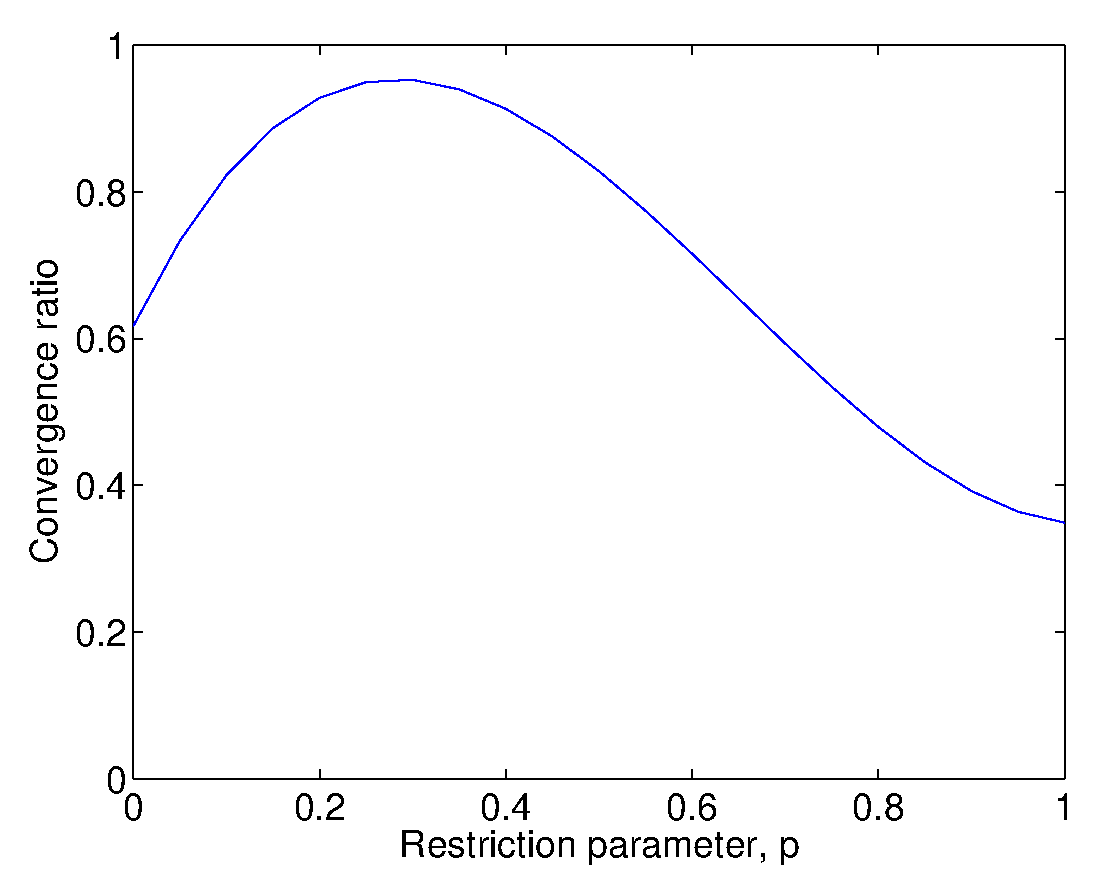
\includegraphics[width=8cm]{gcimages/restrict_p_sm}
    \caption{Средняя скорость сходимости в зависимости от параметра $p$ (тренд)}
    \label{fig:restrict_profit}
\end{figure}

На рисунке~\ref{fig:restrict_profit} проиллюстрировано поведение значения скорости сходимости в зависимости от параметра $p$ (показания усредненны для случайного набора из 500 прогонов иммитационной модели). Под скоростью сходимости понимается отношение продолжительности этапа эксплуатации к общей продолжительности работы системы. Значение $p = 0$ соответствует случаю, когда на переходные правила не накладывается никаких ограничений. Значение $p>0$ - конфигурации, когда некоторая часть переходов случайным образом запрещена для каждого агента. Видно, что для определенного значения ($p=0.3$) коэффициент сходимости увеличивается на $20\%$.

% \subsection{Channel blocking}

\section{Оценка эффективности}

Для анализа производительности, мы проводим моделирование с помощью симулятора, основанном на программном продукте Vienna LTE-A Downlink System Level Simulator (\cite{VTC2010}). Сеть состоит из 2-х уровней - группа малых сот (находящихся внутри помещения) соседствует с базовой макро станцией. Малые соты располагаются в ячейках 5х5 сетки по правилам, указанным в рекомендации консорциума 3GPP ~\cite{R4-092042}. Пользователи равномерно распределены внутри помещения. Предполагается, что каждый пользователь обслуживается базовой станцией с самым сильным сигналом. Рассматриваемые модели распространения сигнала и замирания в канале основаны на рекомендациях ~\cite{R4-092042}. Основные параметры модели, используемые по-умолчанию приведены в таблице~\ref{table:simulation_parameters}.

На рисунке~\ref{fig:fcdf3} показана интегральная функция распределения пропускной способности пользователей для множества прогонов моделирования. Предложенный алгоритм сравнивается с алгоритмом обучения, описанным в~\cite{mab}, где базовые станции принимают решения о распределении поддиапазонов с учетом занятости ресурсов каждой из окружающих сот. Видно, что предлагаемый механизм безопасного сдвига способен увеличить среднюю емкость сети на $8 - 10\%$ без негативного воздействия на честность распределения ресурсов.

\begin{table}
\centering
    \caption{Параметры моделирования}
    \begin{tabular}{|l l|} 
    \hline
    \textbf{Параметр} & \textbf{Описание} \\
    \hline
    \multicolumn{2}{|c|}{\textbf{Детали сценария}} \\
    \hline
    Основой сценарий & 5x5 Grid~\cite{R4-092042} \\
    \hline
    Выходная мощность & 23 дБм \\
    \hline
    Количество базовых станций & 7 \\
    \hline
    Количество пользователей & 28 \\
    \hline
    Планировщик & PF \\
    \hline
    Трафик & BE \\
    \hline
    Тип антенн & Всенаправленные \\
    \hline
    Ширина канала & 20 МГц \\
    \hline
    Продолжительность TTI  & 1 мс \\
    \hline
    Продолжительность симуляции & 300 TTI, 1 ч \\
    \hline
    \multicolumn{2}{|c|}{\textbf{Модель канала}} \\
    \hline
    Несущая частоты & Band 7 \\
    \hline
    Плотность мощности теплового шума  & -174 дБм/Гц \\
    \hline
    Затенение канала & Log-normal, 8 дБ \\
    \hline
    Замирание канала & Плоское замирание \\
    \hline
    \multicolumn{2}{|c|}{\textbf{Параметры алгоритма}} \\
    \hline
    $\alpha$ & 0.1 \\
    \hline
    $\beta$ & 0.05 \\
    \hline
    Коэффициент выкалывания, $p$ & 0.3 \\
    \hline
    \end{tabular}
    \label{table:simulation_parameters}
\end{table}

Эффективность предложенного алгоритма сравненивается с традиционной статической схемой разбиения полосы частот (см., например, \cite{4907410}): 

\textbf{Алгоритм Reuse 1}: каждая базовая станция использует всю доступную полосу пропускания (20 МГц, см. таблицу~\ref{table:simulation_parameters}). Затем ресурсы распределяются между пользователями с помощью пропорционального справедливого планировщика.

\textbf{Алгоритм Reuse 3}: каждой базовой станции выделяется треть всего доступного диапазона. Поддиапазонное распределение настроено так, что соседние базовые станции не используют перекрывающиеся поддиапазоны.

\begin{figure}
    \centering
    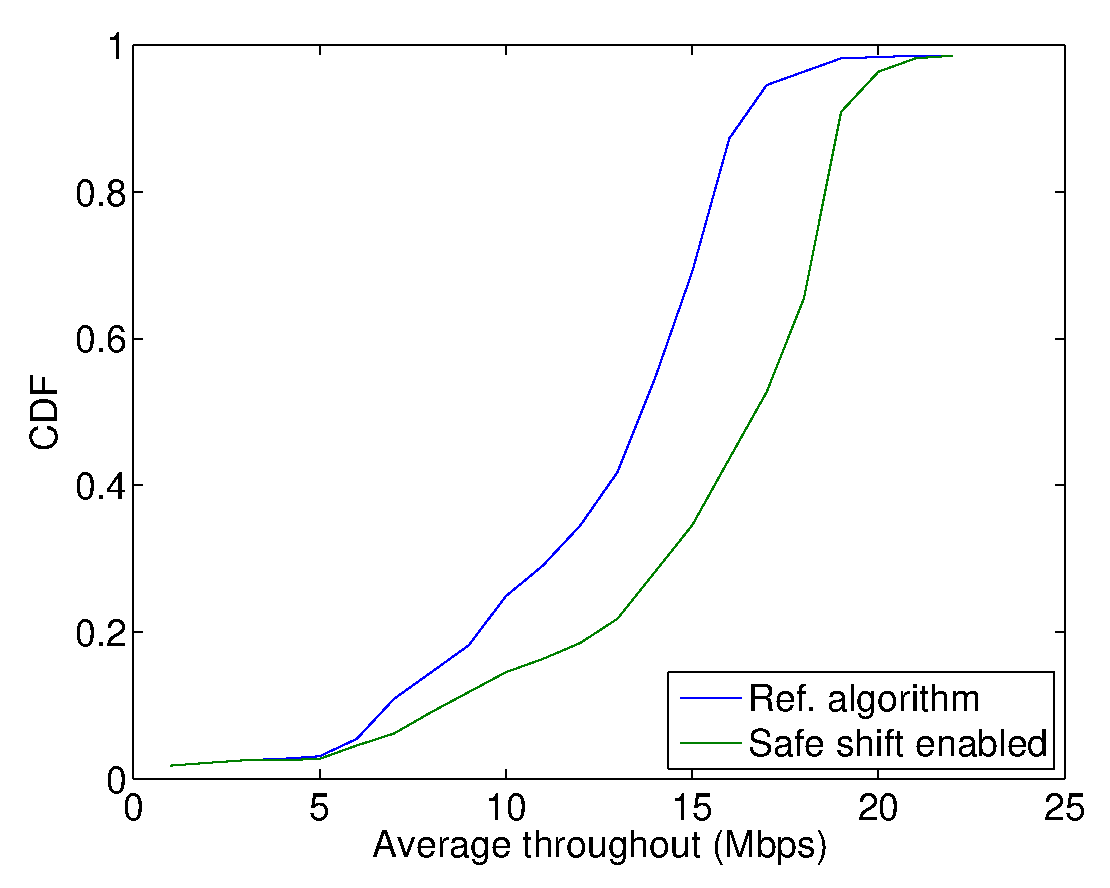
\includegraphics[width=8cm]{gcimages/fcdf3}
    \caption{Функция распределения пропускной способности для пользователей. Алгоритм безопасного сдвига}
    \label{fig:fcdf3}
\end{figure}

На рисунке ~\ref{fig:scdf} показана интегральная функция распределения соотношений сигнал-шум (SINR) для пользователей при использовании предлагаемого алгоритма разделения ресурсов. Значение SINR (соотношения сигнала к интерференции и шуму) рассчитывается для каждого пользователя после выделения ресурсных блоков.
\begin{equation}
    \label{eq:SINR}
    {SINR}_u(b) = \frac{P_u(b) G_u}{\sum_{i \in \eta} P_i(b) G_{u,i} + \sigma^2}
\end{equation}
где $P_u(b)$ - мощность передачи в ресурсном блоке $b$ при обслуживании пользователя $u$; $G_{u,i}$ - ослабление канала между пользователем $u$ и базовой станцией $i$; и $\eta$ - множество соседних базовых станций. Обратим внимание, что $P_i(b) = 0$, если базовая станция $i$ не обслуживает пользователей в поддиапазоне $b$.

\begin{figure}
    \centering
    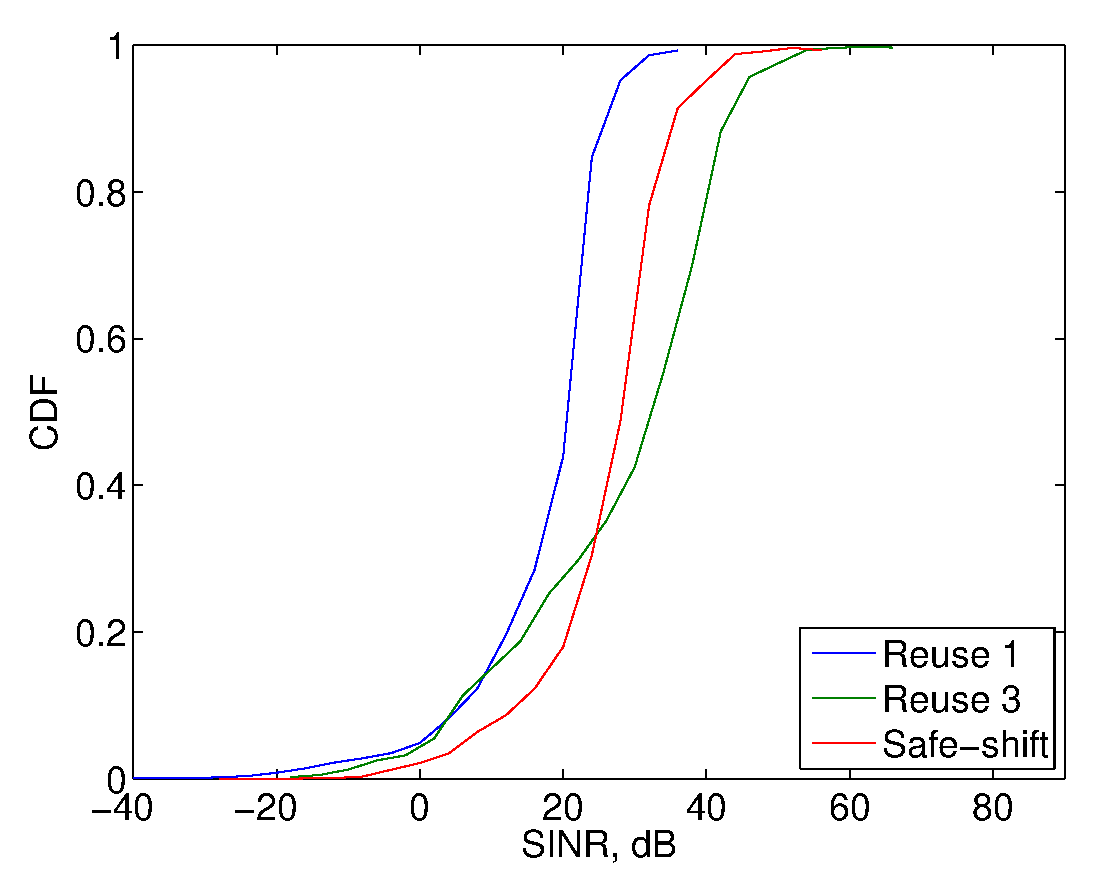
\includegraphics[width=8cm]{gcimages/scdf}
    \caption{Функция распределения соотношений сигнал-шум (SINR) для пользователей сети}
    \label{fig:scdf}
\end{figure}

Из рисунка~\ref{fig:scdf} можно заключить, что предложенный алгоритм способен самостоятельно найти оптимальную схему распределения поддиапазонов и превосходит традиционные централизованные статические схемы разделения ресурсов. Мы также отмечаем, что процедура безопасного сдвига позволяет осуществить исследование без вмешательства в ранее установленную схему распределения ресуров. Это позволяет системе сходится к более выгодной конфигурации без дополнительных затрат, связанных с автономным исследованием. Показано, что предлагаемая процедура позволяет сократить количество шагов случайного исследования среды на $20\%$, при этом оставаясь выше по эффективности на этапе эксплуатации, чем базовый алгоритм.

\section{Обсуждение}
В этой главе мы представили механизм распределения радиоресурсов для координации интерференций между соседними сотами в плотной гетерогенной сети. Он распределяет ресурсы системы на основе мультиагентного параллельного алгоритма обучения. Основной упор делается на сосуществование малых сотовых систем с невзаимодействующей макросредой. Мы также предложили прием для повышения эффективности параллельного обучения за счет снижения эффекта блокировки исследования внешней среды. Воспользовавшись так называемой процедурой безопасного сдвига, мы продемонстрировали способ повышения общей эффективности обучения и обеспечения сосуществования с окружающей средой в многоагентной среде.

Данный алгоритм предполагает гибкий механизм для контроля скорости сходимости в случае разделения радиоресурса на несколько поддиапазонов. В качестве входных данных для алгоритма, мы используем стандартные метрики 3GPP, доступные локально на любой коммерческой малой соте, что делает его легко реализуемым на практике. Вычислительная сложность алгоритма невысока всвязи с итеративным характером получения итогового решения.

Моделирование на системном уровне доказало эффективность предложенного решения в условиях реалистичных сценариев развертывания, рекомендованных консорциумом 3GPP. В нашем исследовании мы показали, что предложенный алгоритм работает в различных разнородных сценариях и превосходит эталонные алгоритмы без негативного влияния на скорость сходимости. Дальнейшие исследования направлены на развитие усовершенствованного алгоритма, способного динамически регулировать размеры поддиапазонов.
